\chapter{细节实现题}
这类题目不考特定的算法,纯粹考察写代码的熟练度。


\section{Reverse Integer (loj7)} %%%%%%%%%%%%%%%%%%%%%%%%%%%%%%
\label{sec:reverse-integer}


\subsubsection{描述}
Reverse digits of an integer.

Example1: x = 123, return 321

Example2: x = -123, return -321


\textbf{Have you thought about this?}

Here are some good questions to ask before coding. Bonus points for you if you have already thought through this!

If the integer's last digit is 0, what should the output be? ie, cases such as 10, 100.

Did you notice that the reversed integer might overflow? Assume the input is a 32-bit integer, then the reverse of 1000000003 overflows. How should you handle such cases?

For the purpose of this problem, assume that your function returns 0 when the reversed integer overflows.

Update (2014-11-10):

Test cases had been added to test the overflow behavior.

\subsubsection{分析}
短小精悍的题,代码也可以写的很短小。


\subsubsection{代码}
\begin{Code}
// LeetCode, Reverse Integer
// 时间复杂度O(logn),空间复杂度O(1)
class Solution {
public:
    int reverse (int x) {
        int r = 0;

        while(x!=0) {
            if(r > INT_MAX/10 || r < INT_MIN/10) {
                return 0;
            }
            r = r * 10 + x % 10;
            x /= 10;
        }
        
        return r;
    }
};
\end{Code}

\subsubsection{代码}
\begin{Code}
// LeetCode, Reverse Integer
// 使用绝对值再判断符号
class Solution {
public:
int reverse(int x) {
        unsigned int val = abs(x);
        unsigned int result = 0;

        while (val) {
            if (result > ((unsigned int)(1 << 31) - 1) / 10)
                return 0;

            result = result * 10 + val % 10;
            val /= 10;
        }

        return (x > 0 ? result : (-1 * result));
    }
};
\end{Code}

\subsubsection{代码}
\begin{Code}
// LeetCode, Reverse Integer
// 使用long
class Solution {
public:
    int reverse(int x) {
        long long ret = 0;
        while (x) {
            int data = x % 10;
            ret = ret * 10 + data;
            if (ret > numeric_limits<int>::max() || ret <= numeric_limits<int>::min()) {
                ret = 0;
                break;
            }
            x /= 10;
        }
        return ret;
    }
};
\end{Code}

\subsubsection{代码}
\begin{Code}
// 不使用long判断溢出
class Solution {
public:
    int reverse(int x) {
        if(x==INT_MIN)
        //solve this situation, we can use x=abs(x)
            return 0;
        int isPositive=1;
        if(x<0)
        {
            x=abs(x);
            isPositive=-1;
        }
        int result=0;
        int int_maxp=INT_MAX/10;
        while(x!=0)
        {
            if (result>int_maxp)
            // don't need to check "result == int_maxp && q > int_maxq"
            // because this can't happen (x is type int)
            {
                result=0;
                break;
            }
            else
                result=10*result+x%10;
            x=x/10;
        }
        result=isPositive*result;
        return result;
    }
};
\end{Code}

\subsubsection{相关题目}
\begindot
\item Palindrome Number, 见 \S \ref{sec:palindrome-number}
\myenddot


\section{Palindrome Number (loj9)} %%%%%%%%%%%%%%%%%%%%%%%%%%%%%%
\label{sec:palindrome-number}


\subsubsection{描述}
Determine whether an integer is a palindrome. Do this without extra space.

\textbf{Some hints:}

Could negative integers be palindromes? (ie, -1)

If you are thinking of converting the integer to string, note the restriction of using extra space.

You could also try reversing an integer. However, if you have solved the problem "Reverse Integer", you know that the reversed integer might overflow. How would you handle such case?

There is a more generic way of solving this problem.


\subsubsection{分析}
首先想到,可以利用上一题,将整数反转,然后与原来的整数比较,是否相等,相等则为 Palindrome 的。可是 reverse()会溢出。

正确的解法是,不断地取第一位和最后一位(10进制下)进行比较,相等则取第二位和倒数第二位,直到完成比较或者中途找到了不一致的位。


\subsubsection{代码}
\begin{Code}
//LeetCode, Palindrome Number
// 时间复杂度O(1),空间复杂度O(1)
class Solution {
public:
    bool isPalindrome(int x) {
        if (x < 0) return false;
        int d = 1; // divisor
        while (x / d >= 10) d *= 10;

        while (x > 0) {
            int q = x / d;  // quotient
            int r = x % 10;   // remainder
            if (q != r) return false;
            // remove the highest bit and remove the lowest bit
            x = x % d / 10;
            d /= 100;
        }
        return true;
    }
};
\end{Code}


\subsubsection{相关题目}
\begindot
\item Reverse Integer, 见 \S \ref{sec:reverse-integer}
\item Valid Palindrome, 见 \S \ref{sec:valid-palindrome}
\myenddot


\section{Insert Interval} %%%%%%%%%%%%%%%%%%%%%%%%%%%%%%
\label{sec:insert-interval}


\subsubsection{描述}
Given a set of non-overlapping intervals, insert a new interval into the intervals (merge if necessary).

You may assume that the intervals were initially sorted according to their start times.

Example 1:
Given intervals \code{[1,3],[6,9]}, insert and merge \code{[2,5]} in as \code{[1,5],[6,9]}.

Example 2:
Given \code{[1,2],[3,5],[6,7],[8,10],[12,16]}, insert and merge \code{[4,9]} in as \code{[1,2],[3,10],[12,16]}.

This is because the new interval \code{[4,9]} overlaps with \code{[3,5],[6,7],[8,10]}.


\subsubsection{分析}
无


\subsubsection{代码}
\begin{Code}
struct Interval {
    int start;
    int end;
    Interval() : start(0), end(0) { }
    Interval(int s, int e) : start(s), end(e) { }
};
 
//LeetCode, Insert Interval
// 时间复杂度O(n),空间复杂度O(1)
class Solution {
public:
    vector<Interval> insert(vector<Interval> &intervals, Interval newInterval) {
        vector<Interval>::iterator it = intervals.begin();
        while (it != intervals.end()) {
            if (newInterval.end < it->start) {
                intervals.insert(it, newInterval);
                return intervals;
            } else if (newInterval.start > it->end) {
                it++;
                continue;
            } else {
                newInterval.start = min(newInterval.start, it->start);
                newInterval.end = max(newInterval.end, it->end);
                it = intervals.erase(it);
            }
        }
        intervals.insert(intervals.end(), newInterval);
        return intervals;
    }
};
\end{Code}


\subsubsection{相关题目}

\begindot
\item Merge Intervals,见 \S \ref{sec:merge-intervals}
\myenddot


\section{Merge Intervals} %%%%%%%%%%%%%%%%%%%%%%%%%%%%%%
\label{sec:merge-intervals}


\subsubsection{描述}
Given a collection of intervals, merge all overlapping intervals.

For example,
Given \code{[1,3],[2,6],[8,10],[15,18]},
return \code{[1,6],[8,10],[15,18]}


\subsubsection{分析}
复用一下Insert Intervals的解法即可,创建一个新的interval集合,然后每次从旧的里面取一个interval出来,然后插入到新的集合中。


\subsubsection{代码}
\begin{Code}
struct Interval {
    int start;
    int end;
    Interval() : start(0), end(0) { }
    Interval(int s, int e) : start(s), end(e) { }
};
 
//LeetCode, Merge Interval
//复用一下Insert Intervals的解法即可
// 时间复杂度O(n1+n2+...),空间复杂度O(1)
class Solution {
public:
    vector<Interval> merge(vector<Interval> &intervals) {
        vector<Interval> result;
        for (int i = 0; i < intervals.size(); i++) {
            insert(result, intervals[i]);
        }
        return result;
    }
private:
    vector<Interval> insert(vector<Interval> &intervals, Interval newInterval) {
        vector<Interval>::iterator it = intervals.begin();
        while (it != intervals.end()) {
            if (newInterval.end < it->start) {
                intervals.insert(it, newInterval);
                return intervals;
            } else if (newInterval.start > it->end) {
                it++;
                continue;
            } else {
                newInterval.start = min(newInterval.start, it->start);
                newInterval.end = max(newInterval.end, it->end);
                it = intervals.erase(it);
            }
        }
        intervals.insert(intervals.end(), newInterval);
        return intervals;
    }
};
\end{Code}


\subsubsection{相关题目}

\begindot
\item Insert Interval,见 \S \ref{sec:insert-interval}
\myenddot


\section{Minimum Window Substring} %%%%%%%%%%%%%%%%%%%%%%%%%%%%%%
\label{sec:minimum-window-substring}


\subsubsection{描述}
Given a string $S$ and a string $T$, find the minimum window in $S$ which will contain all the characters in $T$ in complexity $O(n)$.

For example, \code{S = "ADOBECODEBANC", T = "ABC"}

Minimum window is \code{"BANC"}.

Note:
\begindot
\item If there is no such window in $S$ that covers all characters in $T$, return the emtpy string \code{""}.
\item If there are multiple such windows, you are guaranteed that there will always be only one unique minimum window in $S$.
\myenddot


\subsubsection{分析}
双指针,动态维护一个区间。尾指针不断往后扫,当扫到有一个窗口包含了所有$T$的字符后,然后再收缩头指针,直到不能再收缩为止。最后记录所有可能的情况中窗口最小的


\subsubsection{代码}
\begin{Code}
// LeetCode, Minimum Window Substring
// 时间复杂度O(n),空间复杂度O(1)
class Solution {
public:
    string minWindow(string S, string T) {
        if (S.empty()) return "";
        if (S.size() < T.size()) return "";

        const int ASCII_MAX = 256;
        int appeared_count[ASCII_MAX];
        int expected_count[ASCII_MAX];
        fill(appeared_count, appeared_count + ASCII_MAX, 0);
        fill(expected_count, expected_count + ASCII_MAX, 0);

        for (size_t i = 0; i < T.size(); i++) expected_count[T[i]]++;

        int minWidth = INT_MAX, min_start = 0;  // 窗口大小,起点
        int wnd_start = 0;
        int appeared = 0;  // 完整包含了一个T
        //尾指针不断往后扫
        for (size_t wnd_end = 0; wnd_end < S.size(); wnd_end++) {
            if (expected_count[S[wnd_end]] > 0)  {  // this char is a part of T
                appeared_count[S[wnd_end]]++;
                if (appeared_count[S[wnd_end]] <= expected_count[S[wnd_end]])
                    appeared++;
            }
            if (appeared == T.size()) {  // 完整包含了一个T
                // 收缩头指针
                while (appeared_count[S[wnd_start]] > expected_count[S[wnd_start]]
                        || expected_count[S[wnd_start]] == 0) {
                    appeared_count[S[wnd_start]]--;
                    wnd_start++;
                }
                if (minWidth > (wnd_end - wnd_start + 1)) {
                    minWidth = wnd_end - wnd_start + 1;
                    min_start = wnd_start;
                }
            }
        }

        if (minWidth == INT_MAX) return "";
        else return S.substr(min_start, minWidth);
    }
};
\end{Code}


\subsubsection{相关题目}

\begindot
\item 无
\myenddot


\section{Multiply Strings} %%%%%%%%%%%%%%%%%%%%%%%%%%%%%%
\label{sec:multiply-strings}


\subsubsection{描述}
Given two numbers represented as strings, return multiplication of the numbers as a string.

Note: The numbers can be arbitrarily large and are non-negative.


\subsubsection{分析}
高精度乘法。

常见的做法是将字符转化为一个int,一一对应,形成一个int数组。但是这样很浪费空间,一个int32的最大值是$2^{31}-1=2147483647$,可以与9个字符对应,由于有乘法,减半,则至少可以与4个字符一一对应。一个int64可以与9个字符对应。


\subsubsection{代码1}
\begin{Code}
// LeetCode, Multiply Strings
// @author 连城 (http://weibo.com/lianchengzju)
// 一个字符对应一个int
// 时间复杂度O(n*m),空间复杂度O(n+m)
typedef vector<int> bigint;

bigint make_bigint(string const& repr) {
    bigint n;
    transform(repr.rbegin(), repr.rend(), back_inserter(n),
            [](char c) { return c - '0'; });
    return n;
}

string to_string(bigint const& n) {
    string str;
    transform(find_if(n.rbegin(), prev(n.rend()),
            [](char c) { return c > '\0'; }), n.rend(), back_inserter(str),
            [](char c) { return c + '0'; });
    return str;
}

bigint operator*(bigint const& x, bigint const& y) {
    bigint z(x.size() + y.size());

    for (size_t i = 0; i < x.size(); ++i)
        for (size_t j = 0; j < y.size(); ++j) {
            z[i + j] += x[i] * y[j];
            z[i + j + 1] += z[i + j] / 10;
            z[i + j] %= 10;
        }

    return z;
}

class Solution {
public:
    string multiply(string num1, string num2) {
        return to_string(make_bigint(num1) * make_bigint(num2));
    }
};
\end{Code}


\subsubsection{代码2}
\begin{Code}
// LeetCode, Multiply Strings
// 9个字符对应一个int64_t
// 时间复杂度O(n*m/81),空间复杂度O((n+m)/9)
/** 大整数类. */
class BigInt {
public:
    /**
     * @brief 构造函数,将字符串转化为大整数.
     * @param[in] s 输入的字符串
     * @return 无
     */
    BigInt(string s) {
        vector<int64_t> result;
        result.reserve(s.size() / RADIX_LEN + 1);

        for (int i = s.size(); i > 0; i -= RADIX_LEN) {  // [i-RADIX_LEN, i)
            int temp = 0;
            const int low = max(i - RADIX_LEN, 0);
            for (int j = low; j < i; j++) {
                temp = temp * 10 + s[j] - '0';
            }
            result.push_back(temp);
        }
        elems = result;
    }
    /**
     * @brief 将整数转化为字符串.
     * @return 字符串
     */
    string toString() {
        stringstream result;
        bool started = false; // 用于跳过前导0
        for (auto i = elems.rbegin(); i != elems.rend(); i++) {
            if (started) { // 如果多余的0已经都跳过,则输出
                result << setw(RADIX_LEN) << setfill('0') << *i;
            } else {
                result << *i;
                started = true; // 碰到第一个非0的值,就说明多余的0已经都跳过
            }
        }

        if (!started) return "0"; // 当x全为0时
        else return result.str();
    }

    /**
     * @brief 大整数乘法.
     * @param[in] x x
     * @param[in] y y
     * @return 大整数
     */
    static BigInt multiply(const BigInt &x, const BigInt &y) {
        vector<int64_t> z(x.elems.size() + y.elems.size(), 0);

        for (size_t i = 0; i < y.elems.size(); i++) {
            for (size_t j = 0; j < x.elems.size(); j++) { // 用y[i]去乘以x的各位
                //  两数第i, j位相乘,累加到结果的第i+j位
                z[i + j] += y.elems[i] * x.elems[j];

                if (z[i + j] >= BIGINT_RADIX) { //  看是否要进位
                    z[i + j + 1] += z[i + j] / BIGINT_RADIX; //  进位
                    z[i + j] %= BIGINT_RADIX;
                }
            }
        }
        while (z.back() == 0) z.pop_back();  // 没有进位,去掉最高位的0
        return BigInt(z);
    }

private:
    typedef long long int64_t;
    /** 一个数组元素对应9个十进制位,即数组是亿进制的
     * 因为 1000000000 * 1000000000 没有超过 2^63-1
     */
    const static int BIGINT_RADIX = 1000000000;
    const static int RADIX_LEN = 9;
    /** 万进制整数. */
    vector<int64_t> elems;
    BigInt(const vector<int64_t> num) : elems(num) {}
};


class Solution {
public:
    string multiply(string num1, string num2) {
        BigInt x(num1);
        BigInt y(num2);
        return BigInt::multiply(x, y).toString();
    }
};
\end{Code}


\subsubsection{相关题目}

\begindot
\item 无
\myenddot


\section{Substring with Concatenation of All Words} %%%%%%%%%%%%%%%%%%%%%%%%%%%%%%
\label{sec:substring-with-concatenation-of-all-words}


\subsubsection{描述}
You are given a string, $S$, and a list of words, $L$, that are all of the same length. Find all starting indices of substring(s) in $S$ that is a concatenation of each word in $L$ exactly once and without any intervening characters.

For example, given: 
\begin{Code}
S: "barfoothefoobarman"
L: ["foo", "bar"]
\end{Code}

You should return the indices: \code{[0,9]}.(order does not matter).


\subsubsection{分析}
无


\subsubsection{代码}
\begin{Code}
// LeetCode, Substring with Concatenation of All Words
// 时间复杂度O(n*m),空间复杂度O(m)
class Solution {
public:
    vector<int> findSubstring(string s, vector<string>& dict) {
        size_t wordLength = dict.front().length();
        size_t catLength = wordLength * dict.size();
        vector<int> result;

        if (s.length() < catLength) return result;

        unordered_map<string, int> wordCount;

        for (auto const& word : dict) ++wordCount[word];

        for (auto i = begin(s); i <= prev(end(s), catLength); ++i) {
            unordered_map<string, int> unused(wordCount);

            for (auto j = i; j != next(i, catLength); j += wordLength) {
                auto pos = unused.find(string(j, next(j, wordLength)));

                if (pos == unused.end() || pos->second == 0) break;

                if (--pos->second == 0) unused.erase(pos);
            }

            if (unused.size() == 0) result.push_back(distance(begin(s), i));
        }

        return result;
    }
};
\end{Code}


\subsubsection{相关题目}

\begindot
\item 无
\myenddot


\section{Pascal's Triangle (loj118)} %%%%%%%%%%%%%%%%%%%%%%%%%%%%%%
\label{sec:pascals-triangle}


\subsubsection{描述}
Given $numRows$, generate the first $numRows$ of Pascal's triangle.

For example, given $numRows = 5$,

Return
\begin{Code}
[
     [1],
    [1,1],
   [1,2,1],
  [1,3,3,1],
 [1,4,6,4,1]
]
\end{Code}


\subsubsection{分析}
本题可以用队列,计算下一行时,给上一行左右各加一个0,然后下一行的每个元素,就等于左上角和右上角之和。

另一种思路,下一行第一个元素和最后一个元素赋值为1,中间的每个元素,等于上一行的左上角和右上角元素之和。

\subsubsection{从左到右}
\begin{Code}
// LeetCode, Pascal's Triangle
// 时间复杂度O(n^2),空间复杂度O(n)
class Solution {
public:
    vector<vector<int>> generate(int numRows) {
        vector<vector<int>> result;
        if(numRows == 0) return result;

        result.push_back(vector<int>(1,1)); //first row

        for(int i = 2; i <= numRows; ++i) {
            vector<int> current(i,1);  // 本行
            const vector<int> &prev = result[i-2];  // 上一行

            for(int j = 1; j < i - 1; ++j) {
                current[j] = prev[j-1] + prev[j]; // 左上角和右上角之和
            }
            result.push_back(current);
        }
        return result;
    }
};
\end{Code}

\subsubsection{从左到右}
\begin{Code}
class Solution {
public:
    vector<vector<int>> generate(int numRows) {
        vector<vector<int>> r(numRows);
        for (int i = 0; i < numRows; i++) {
            r[i].resize(i + 1);
            r[i][0] = r[i][i] = 1;
            for (int j = 1; j < i; j++)
                r[i][j] = r[i - 1][j - 1] + r[i - 1][j];
        }
        return r;
    }
};
\end{Code}

\subsubsection{从右到左}
\begin{Code}
// LeetCode, Pascal's Triangle
// 时间复杂度O(n^2),空间复杂度O(n)
class Solution {
public:
    vector<vector<int> > generate(int numRows) {
        vector<vector<int> > result;
        vector<int> array;
        for (int i = 1; i <= numRows; i++) {
            for (int j = i - 2; j > 0; j--) {
                array[j] = array[j - 1] + array[j];
            }
            array.push_back(1);
            result.push_back(array);
        }
        return result;
    }
};
\end{Code}


\subsubsection{相关题目}
\begindot
\item Pascal's Triangle II,见 \S \ref{sec:pascals-triangle-ii}
\myenddot


\section{Pascal's Triangle II} %%%%%%%%%%%%%%%%%%%%%%%%%%%%%%
\label{sec:pascals-triangle-ii}


\subsubsection{描述}
Given an index $k$, return the $k^{th}$ row of the Pascal's triangle.

For example, given $k = 3$,

Return \code{[1,3,3,1]}.

Note: Could you optimize your algorithm to use only $O(k)$ extra space?


\subsubsection{分析}
滚动数组。


\subsubsection{代码}

\begin{Code}
// LeetCode, Pascal's Triangle II
// 滚动数组,时间复杂度O(n^2),空间复杂度O(n)
class Solution {
public:
	vector<int> getRow(int rowIndex) {
		vector<int> array;
		for (int i = 0; i <= rowIndex; i++) {
			for (int j = i - 1; j > 0; j--){
				array[j] = array[j - 1] + array[j];
			}
			array.push_back(1);
		}
		return array;
	}
};
\end{Code}


\subsubsection{相关题目}
\begindot
\item Pascal's Triangle,见 \S \ref{sec:pascals-triangle}
\myenddot


\section{Spiral Matrix} %%%%%%%%%%%%%%%%%%%%%%%%%%%%%%
\label{sec:spiral-matrix}


\subsubsection{描述}
Given a matrix of $m \times n$ elements ($m$ rows, $n$ columns), return all elements of the matrix in spiral order.

For example,
Given the following matrix:
\begin{Code}
[
 [ 1, 2, 3 ],
 [ 4, 5, 6 ],
 [ 7, 8, 9 ]
]
\end{Code}
You should return \fn{[1,2,3,6,9,8,7,4,5]}.


\subsubsection{分析}
模拟。

\subsubsection{代码}
\begin{Code}
// LeetCode, Spiral Matrix
// @author 龚陆安 (http://weibo.com/luangong)
// 时间复杂度O(n^2),空间复杂度O(1)
class Solution {
public:
    vector<int> spiralOrder(vector<vector<int> >& matrix) {
        vector<int> result;
        if (matrix.empty()) return result;
        int beginX = 0, endX = matrix[0].size() - 1;
        int beginY = 0, endY = matrix.size() - 1;
        while (true) {
            // From left to right
            for (int j = beginX; j <= endX; ++j) result.push_back(matrix[beginY][j]);
            if (++beginY > endY) break;
            // From top to bottom
            for (int i = beginY; i <= endY; ++i) result.push_back(matrix[i][endX]);
            if (beginX > --endX) break;
            // From right to left
            for (int j = endX; j >= beginX; --j) result.push_back(matrix[endY][j]);
            if (beginY > --endY) break;
            // From bottom to top
            for (int i = endY; i >= beginY; --i) result.push_back(matrix[i][beginX]);
            if (++beginX > endX) break;
        }
        return result;
    }
};
\end{Code}


\subsubsection{相关题目}
\begindot
\item Spiral Matrix II ,见 \S \ref{sec:spiral-matrix-ii}
\myenddot


\section{Spiral Matrix II} %%%%%%%%%%%%%%%%%%%%%%%%%%%%%%
\label{sec:spiral-matrix-ii}


\subsubsection{描述}
Given an integer $n$, generate a square matrix filled with elements from 1 to $n^2$ in spiral order.

For example,
Given $n = 3$,

You should return the following matrix:
\begin{Code}
[
 [ 1, 2, 3 ],
 [ 8, 9, 4 ],
 [ 7, 6, 5 ]
]
\end{Code}


\subsubsection{分析}
这题比上一题要简单。


\subsubsection{代码1}
\begin{Code}
// LeetCode, Spiral Matrix II
// 时间复杂度O(n^2),空间复杂度O(n^2)
class Solution {
public:
    vector<vector<int> > generateMatrix(int n) {
        vector<vector<int> > matrix(n, vector<int>(n));
        int begin = 0, end = n - 1;
        int num = 1;

        while (begin < end) {
            for (int j = begin; j < end; ++j) matrix[begin][j] = num++;
            for (int i = begin; i < end; ++i) matrix[i][end] = num++;
            for (int j = end; j > begin; --j) matrix[end][j] = num++;
            for (int i = end; i > begin; --i) matrix[i][begin] = num++;
            ++begin;
            --end;
        }

        if (begin == end) matrix[begin][begin] = num;

        return matrix;
    }
};
\end{Code}


\subsubsection{代码2}
\begin{Code}
// LeetCode, Spiral Matrix II
// @author 龚陆安 (http://weibo.com/luangong)
// 时间复杂度O(n^2),空间复杂度O(n^2)
class Solution {
public:
    vector<vector<int> > generateMatrix(int n) {
        vector< vector<int> > matrix(n, vector<int>(n));
        if (n == 0) return matrix;
        int beginX = 0, endX = n - 1;
        int beginY = 0, endY = n - 1;
        int num = 1;
        while (true) {
            for (int j = beginX; j <= endX; ++j) matrix[beginY][j] = num++;
            if (++beginY > endY) break;

            for (int i = beginY; i <= endY; ++i) matrix[i][endX] = num++;
            if (beginX > --endX) break;

            for (int j = endX; j >= beginX; --j) matrix[endY][j] = num++;
            if (beginY > --endY) break;

            for (int i = endY; i >= beginY; --i) matrix[i][beginX] = num++;
            if (++beginX > endX) break;
        }
        return matrix;
    }
};
\end{Code}


\subsubsection{相关题目}
\begindot
\item Spiral Matrix, 见 \S \ref{sec:spiral-matrix}
\myenddot


\section{ZigZag Conversion} %%%%%%%%%%%%%%%%%%%%%%%%%%%%%%
\label{sec:zigzag-conversion}


\subsubsection{描述}
The string \code{"PAYPALISHIRING"} is written in a zigzag pattern on a given number of rows like this: (you may want to display this pattern in a fixed font for better legibility)

\begin{Code}
P   A   H   N
A P L S I I G
Y   I   R
\end{Code}

And then read line by line: \code{"PAHNAPLSIIGYIR"}

Write the code that will take a string and make this conversion given a number of rows:
\begin{Code}
string convert(string text, int nRows);
\end{Code}
\code{convert("PAYPALISHIRING", 3)} should return \code{"PAHNAPLSIIGYIR"}.


\subsubsection{分析}
要找到数学规律。真正面试中,不大可能出这种问题。

n=4:
\begin{Code}
P     I     N
A   L S   I G
Y A   H R
P     I
\end{Code}

n=5:
\begin{Code}
P       H
A     S I
Y   I   R
P L     I  G
A       N
\end{Code}

所以,对于每一层垂直元素的坐标 $(i,j)= (j+1 )*n +i$;对于每两层垂直元素之间的插入元素(斜对角元素),$(i,j)= (j+1)*n -i$


\subsubsection{代码}
\begin{Code}
// LeetCode, ZigZag Conversion
// 时间复杂度O(n),空间复杂度O(1)
class Solution {
public:
    string convert(string s, int nRows) {
        if (nRows <= 1 || s.size() <= 1) return s;
        string result;
        for (int i = 0; i < nRows; i++) {
            for (int j = 0, index = i; index < s.size();
                    j++, index = (2 * nRows - 2) * j + i) {
                result.append(1, s[index]);  // 垂直元素
                if (i == 0 || i == nRows - 1) continue;   // 斜对角元素
                if (index + (nRows - i - 1) * 2 < s.size())
                    result.append(1, s[index + (nRows - i - 1) * 2]);
            }
        }
        return result;
    }
};
\end{Code}


\subsubsection{相关题目}
\begindot
\item 无
\myenddot


\section{Divide Two Integers} %%%%%%%%%%%%%%%%%%%%%%%%%%%%%%
\label{sec:divide-two-integers}


\subsubsection{描述}
Divide two integers without using multiplication, division and mod operator.


\subsubsection{分析}
不能用乘、除和取模,那剩下的,还有加、减和位运算。

最简单的方法,是不断减去被除数。在这个基础上,可以做一点优化,每次把被除数翻倍,从而加速。


\subsubsection{代码1}
\begin{Code}
// LeetCode, Divide Two Integers
// 时间复杂度O(logn),空间复杂度O(1)
class Solution {
public:
    int divide(int dividend, int divisor) {
        // 当 dividend = INT_MIN时,-dividend会溢出,所以用 long long
        long long a = dividend >= 0 ? dividend : -(long long)dividend;
        long long b = divisor >= 0 ? divisor : -(long long)divisor;

        // 当 dividend = INT_MIN时,divisor = -1时,结果会溢出,所以用 long long
        long long result = 0;
        while (a >= b) {
            long long c = b;
            for (int i = 0; a >= c; ++i, c <<= 1) {
                a -= c;
                result += 1 << i;
            }
        }

        return ((dividend^divisor) >> 31) ? (-result) : (result);
    }
};
\end{Code}


\subsubsection{代码2}
\begin{Code}
// LeetCode, Divide Two Integers
// 时间复杂度O(logn),空间复杂度O(1)
class Solution {
public:
    int divide(int dividend, int divisor) {
        int result = 0; // 当 dividend = INT_MIN时,divisor = -1时,结果会溢出
        const bool sign = (dividend > 0 && divisor < 0) ||
                (dividend < 0 && divisor > 0); // 异号

        // 当 dividend = INT_MIN时,-dividend会溢出,所以用 unsigned int
        unsigned int a = dividend >= 0 ? dividend : -dividend;
        unsigned int b = divisor >= 0 ? divisor : -divisor;

        while (a >= b) {
            int multi = 1;
            unsigned int bb = b;
            while (a >= bb) {
                a -= bb;
                result += multi;

                if (bb < INT_MAX >> 1) { // 防止溢出
                    bb += bb;
                    multi += multi;
                }
            }
        }
        if (sign) return -result;
        else return result;
    }
};
\end{Code}


\subsubsection{相关题目}
\begindot
\item 无
\myenddot


\section{Text Justification} %%%%%%%%%%%%%%%%%%%%%%%%%%%%%%
\label{sec:text-justification}


\subsubsection{描述}
Given an array of words and a length $L$, format the text such that each line has exactly $L$ characters and is fully (left and right) justified.

You should pack your words in a greedy approach; that is, pack as many words as you can in each line. Pad extra spaces \fn{' '} when necessary so that each line has exactly $L$ characters.

Extra spaces between words should be distributed as evenly as possible. If the number of spaces on a line do not divide evenly between words, the empty slots on the left will be assigned more spaces than the slots on the right.

For the last line of text, it should be left justified and no extra space is inserted between words.

For example, \\
words: \code{["This", "is", "an", "example", "of", "text", "justification."]} \\
L: 16.

Return the formatted lines as:
\begin{Code}
[
   "This    is    an",
   "example  of text",
   "justification.  "
]
\end{Code}

Note: Each word is guaranteed not to exceed $L$ in length.

Corner Cases:
\begindot
\item A line other than the last line might contain only one word. What should you do in this case?
\item In this case, that line should be left
\myenddot


\subsubsection{分析}
无


\subsubsection{代码}
\begin{Code}
// LeetCode, Text Justification
// 时间复杂度O(n),空间复杂度O(1)
class Solution {
public:
    vector<string> fullJustify(vector<string> &words, int L) {
        vector<string> result;
        const int n = words.size();
        int begin = 0, len = 0; // 当前行的起点,当前长度
        for (int i = 0; i < n; ++i) {
            if (len + words[i].size() + (i - begin) > L) {
                result.push_back(connect(words, begin, i - 1, len, L, false));
                begin = i;
                len = 0;
            }
            len += words[i].size();
        }
        // 最后一行不足L
        result.push_back(connect(words, begin, n - 1, len, L, true));
        return result;
    }
    /**
     * @brief 将 words[begin, end] 连成一行
     * @param[in] words 单词列表
     * @param[in] begin 开始
     * @param[in] end 结束
     * @param[in] len words[begin, end]所有单词加起来的长度
     * @param[in] L 题目规定的一行长度
     * @param[in] is_last 是否是最后一行
     * @return 对齐后的当前行
     */
    string connect(vector<string> &words, int begin, int end,
            int len, int L, bool is_last) {
        string s;
        int n = end - begin + 1;
        for (int i = 0; i < n; ++i) {
            s += words[begin + i];
            addSpaces(s, i, n - 1, L - len, is_last);
        }

        if (s.size() < L) s.append(L - s.size(), ' ');
        return s;
    }

    /**
     * @brief 添加空格.
     * @param[inout]s 一行
     * @param[in] i 当前空隙的序号
     * @param[in] n 空隙总数
     * @param[in] L 总共需要添加的空额数
     * @param[in] is_last 是否是最后一行
     * @return 无
     */
    void addSpaces(string &s, int i, int n, int L, bool is_last) {
        if (n < 1 || i > n - 1) return;
        int spaces = is_last ? 1 : (L / n + (i < (L % n) ? 1 : 0));
        s.append(spaces, ' ');
    }
};
\end{Code}


\subsubsection{相关题目}
\begindot
\item 无
\myenddot


\section{Max Points on a Line} %%%%%%%%%%%%%%%%%%%%%%%%%%%%%%
\label{sec:Max-Points-on-a-Line}


\subsubsection{描述}
Given $n$ points on a 2D plane, find the maximum number of points that lie on the same straight line.


\subsubsection{分析}
暴力枚举法。两点决定一条直线,$n$个点两两组合,可以得到$\dfrac{1}{2}n(n+1)$条直线,对每一条直线,判断$n$个点是否在该直线上,从而可以得到这条直线上的点的个数,选择最大的那条直线返回。复杂度$O(n^3)$。

上面的暴力枚举法以“边”为中心,再看另一种暴力枚举法,以每个“点”为中心,然后遍历剩余点,找到所有的斜率,如果斜率相同,那么一定共线对每个点,用一个哈希表,key为斜率,value为该直线上的点数,计算出哈希表后,取最大值,并更新全局最大值,最后就是结果。时间复杂度$O(n^2)$,空间复杂度$O(n)$。


\subsubsection{以边为中心}
\begin{Code}
// LeetCode, Max Points on a Line
// 暴力枚举法,以边为中心,时间复杂度O(n^3),空间复杂度O(1)
class Solution {
public:
    int maxPoints(vector<Point> &points) {
        if (points.size() < 3) return points.size();
        int result = 0;

        for (int i = 0; i < points.size() - 1; i++) {
            for (int j = i + 1; j < points.size(); j++) {
                int sign = 0;
                int a, b, c;
                if (points[i].x == points[j].x) sign = 1;
                else {
                    a = points[j].x - points[i].x;
                    b = points[j].y - points[i].y;
                    c = a * points[i].y - b * points[i].x;
                }
                int count = 0;
                for (int k = 0; k < points.size(); k++) {
                    if ((0 == sign && a * points[k].y == c +  b * points[k].x) || 
                        (1 == sign&&points[k].x == points[j].x)) 
                        count++;
                }
                if (count > result) result = count;
            }
        }
        return result;
    }
};
\end{Code}


\subsubsection{以点为中心}
\begin{Code}
// LeetCode, Max Points on a Line
// 暴力枚举,以点为中心,时间复杂度O(n^2),空间复杂度O(n)
class Solution {
public:
    int maxPoints(vector<Point> &points) {
        if (points.size() < 3) return points.size();
        int result = 0;

        unordered_map<double, int> slope_count;
        for (int i = 0; i < points.size()-1; i++) {
            slope_count.clear();
            int samePointNum = 0; // 与i重合的点
            int point_max = 1;    // 和i共线的最大点数

            for (int j = i + 1; j < points.size(); j++) {
                double slope; // 斜率
                if (points[i].x == points[j].x) {
                    slope = std::numeric_limits<double>::infinity();
                    if (points[i].y == points[j].y) {
                        ++ samePointNum;
                        continue;
                    }
                } else {
                    slope = 1.0 * (points[i].y - points[j].y) / 
                        (points[i].x - points[j].x);
                }

                int count = 0;
                if (slope_count.find(slope) != slope_count.end())
                    count = ++slope_count[slope];
                else {
                    count = 2;
                    slope_count[slope] = 2;
                }

                if (point_max < count) point_max = count;
            }
            result = max(result, point_max + samePointNum);
        }
        return result;
    }
};
\end{Code}


\subsubsection{相关题目}
\begindot
\item 无
\myenddot

\section{Rectangle Area (loj223)} %%%%%%%%%%%%%%%%%%%%%%%%%%%%%%
\label{sec:Rectangle-Area}

\subsubsection{描述}
Find the total area covered by two \textbf{rectilinear} rectangles in a \textbf{2D} plane.

Each rectangle is defined by its bottom left corner and top right corner as shown in the figure.

\begin{center}
    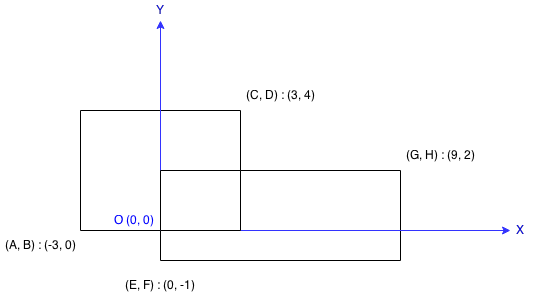
\includegraphics[width=0.8\textwidth]{rectangle-area.png}\\
    \figcaption{Rectangle Area}\label{fig:rectangle-area}
\end{center}

Assume that the total area is never beyond the maximum possible value of \fn{int}.

\subsubsection{分析}
Instead of checking whether the rectangles overlap, I max right with left (and top with bottom). Haven't seen that in other solutions.

\subsubsection{代码}
\begin{Code}
class Solution {
    public:
    int computeArea(int A, int B, int C, int D, int E, int F, int G, int H) {
        int left = max(A,E), right = max(min(C,G), left);
        int bottom = max(B,F), top = max(min(D,H), bottom);
        return (C-A)*(D-B) - (right-left)*(top-bottom) + (G-E)*(H-F);
    }
}
\end{Code}

\subsubsection{分析和代码}
The original version wasn't passing anymore because of new test cases that cause overflow. So now we're avoiding computing the differences below if the result will be negative. This avoids overflow in cases where the rectangles are far apart. It looks like this is basically the same thing that @shw1500 was suggesting, but you don't need the extra max function on the outside.

The return statement is based on comments from @StefanPochmann. We want to avoid forming the sum area(R1) + area(R2). This avoids overflow in cases where area(R1) + area(R2) will overflow, but area(R1) + area(R2) - overlap(R1, R2) fits in an int. There aren't any test cases for this. Add some maybe? Edit: There are test cases for this, but the overflow didn't matter.

New version- avoids overflow when area(R1) + area(R2) overflows but the answer shouldn't.

\begin{Code}
class Solution {
    public:
    int computeArea(int A, int B, int C, int D, int E, int F, int G, int H) {
        int overlap_width = min(C, G) > max(A, E) ? min(C, G) - max(A, E) : 0; 
        int overlap_height = min(D, H) > max(B, F) ? min(D, H) - max(B, F) : 0;
        // order avoids overflow
        return ((C - A) * (D - B) - overlap_width * overlap_height) + (G - E) * (H - F); 
    }
};
\end{Code}

Second version- avoids overflow when rectangles are far apart

\begin{Code}
class Solution {
    public:
    int computeArea(int A, int B, int C, int D, int E, int F, int G, int H) {
        int overlap_width = min(C, G) > max(A, E) ? min(C, G) - max(A, E) : 0; 
        int overlap_height = min(D, H) > max(B, F) ? min(D, H) - max(B, F) : 0;
        return (C - A) * (D - B) + (G - E) * (H - F) - overlap_width * overlap_height;
    }
};
\end{Code}

Old version- overflows for some inputs where the rectangles are far apart.

\begin{Code}
class Solution {
    public:
    int computeArea(int A, int B, int C, int D, int E, int F, int G, int H) {
        int overlap_width = max(min(C, G) - max(A, E), 0);
        int overlap_height = max(min(D, H) - max(B, F), 0);
        return (C - A) * (D - B) + (G - E) * (H - F) - overlap_width * overlap_height;
    }
};
\end{Code}

\subsubsection{相关题目}
\begindot
\item 无
\myenddot

\section{Number of 1 Bits (loj191)} %%%%%%%%%%%%%%%%%%%%%%%%%%%%%%
\label{sec:number-of-1-bits}

\subsubsection{描述}

Write a function that takes an unsigned integer and returns the number of ’1' bits it has (also known as the Hamming weight).

For example, the 32-bit integer ’11' has binary representation \fn{00000000000000000000000000001011}, so the function should return 3.

\subsubsection{分析}

n \& (n - 1) drops the lowest set bit. It's a neat little bit trick.

Let's use n = 00101100 as an example. This binary representation has three 1s.

If n = 00101100, then n - 1 = 00101011, so n \& (n - 1) = 00101100 \& 00101011 = 00101000. Count = 1.

If n = 00101000, then n - 1 = 00100111, so n \& (n - 1) = 00101000 \& 00100111 = 00100000. Count = 2.

If n = 00100000, then n - 1 = 00011111, so n \& (n - 1) = 00100000 \& 00011111 = 00000000. Count = 3.

n is now zero, so the while loop ends, and the final count (the numbers of set bits) is returned.

\subsubsection{代码}
\begin{Code}
class Solution {
public:
    int hammingWeight(uint32_t n) {
        int count = 0;
        while (n) {
            n &= (n - 1);
            count++;
        }
        return count;
    }
};
\end{Code}

\subsubsection{代码}
\begin{Code}
class Solution {
public:
    int hammingWeight(uint32_t n) {
        int sum=0;
        while(n) {
            if(n % 2 == 1) sum++;
            n /= 2; 
        }
        return sum;
    }
};
\end{Code}

\subsubsection{相关题目}

\begindot
\item 无
\myenddot